\documentclass[aps,twocolumn,secnumarabic,balancelastpage,amsmath,amssymb,nofootinbib]{revtex4}
% \documentclass[aps,twocolumn,secnumarabic,balancelastpage,amsmath,amssymb,nofootinbib]{revtex4}

% Documentclass Options

% nobalancelastpage doesn't attempt to equalize the lengths of the two columns
% on the last page as might be desired in a journal where articles follow one
% another closely
% amsmath and amssymb are necessary for the subequations environment among
% others secnumarabic identifies sections by number to aid electronic review
% and commentary. nofootinbib forces footnotes to occur on the page where they
% are first referenced and not in the bibliography

% \usepackage{lgrind}        % convert program listings to a form includable in a LaTeX document
\usepackage{chapterbib}    % allows a bibliography for each chapter (each labguide has it's own)
\usepackage{color}         % produces boxes or entire pages with colored backgrounds
\usepackage{graphics}      % standard graphics specifications
\usepackage[pdftex]{graphicx}      % alternative graphics specifications
\usepackage{longtable}     % helps with long table options
\usepackage{epsf}          % old package handles encapsulated post script issues
\usepackage{bm}            % special 'bold-math' package
\usepackage{tikz}
\usepackage{asymptote}     % For typesetting of mathematical illustrations
\usepackage{subfigure}

% \usepackage{thumbpdf}

\usepackage[colorlinks=true]{hyperref}  % this package should be added after all others
% use as follows: \url{http://web.mit.edu/8.13}
\newcommand{\drelectron}[1]{\node at #1 [circle, draw, inner sep=0pt, minimum size=1pt] {\_}}
\newcommand{\ud}{\mathrm{d}}
\newcommand{\ue}{\mathrm{e}}
\newcommand{\ui}{\mathrm{i}}
\newcommand{\res}{\mathrm{Res}}
\newcommand{\Tr}{\mathrm{Tr}}
\newcommand{\dsum}{\displaystyle\sum}
\newcommand{\dprod}{\displaystyle\prod}
\newcommand{\dlim}{\displaystyle\lim}
\newcommand{\dint}{\displaystyle\int}
\newcommand{\fsno}[1]{{\!\not\!{#1}}}
\newcommand{\eqar}[1]
{
  \begin{align*}
    #1
  \end{align*}
}
\newcommand{\texp}[2]{\ensuremath{{#1}\times10^{#2}}}
\newcommand{\dexp}[2]{\ensuremath{{#1}\cdot10^{#2}}}
\newcommand{\eval}[2]{{\left.{#1}\right|_{#2}}}
\newcommand{\paren}[1]{{\left({#1}\right)}}
\newcommand{\lparen}[1]{{\left({#1}\right.}}
\newcommand{\rparen}[1]{{\left.{#1}\right)}}
\newcommand{\abs}[1]{{\left|{#1}\right|}}
\newcommand{\sqr}[1]{{\left[{#1}\right]}}
\newcommand{\crly}[1]{{\left\{{#1}\right\}}}
\newcommand{\angl}[1]{{\left\langle{#1}\right\rangle}}
\newcommand{\tpdiff}[4][{}]{{\paren{\frac{\partial^{#1} {#2}}{\partial {#3}{}^{#1}}}_{#4}}}
\newcommand{\tpsdiff}[4][{}]{{\paren{\frac{\partial^{#1}}{\partial {#3}{}^{#1}}{#2}}_{#4}}}
\newcommand{\pdiff}[3][{}]{{\frac{\partial^{#1} {#2}}{\partial {#3}{}^{#1}}}}
\newcommand{\diff}[3][{}]{{\frac{\ud^{#1} {#2}}{\ud {#3}{}^{#1}}}}
\newcommand{\psdiff}[3][{}]{{\frac{\partial^{#1}}{\partial {#3}{}^{#1}} {#2}}}
\newcommand{\sdiff}[3][{}]{{\frac{\ud^{#1}}{\ud {#3}{}^{#1}} {#2}}}
\newcommand{\tpddiff}[4][{}]{{\left(\dfrac{\partial^{#1} {#2}}{\partial {#3}{}^{#1}}\right)_{#4}}}
\newcommand{\tpsddiff}[4][{}]{{\paren{\dfrac{\partial^{#1}}{\partial {#3}{}^{#1}}{#2}}_{#4}}}
\newcommand{\pddiff}[3][{}]{{\dfrac{\partial^{#1} {#2}}{\partial {#3}{}^{#1}}}}
\newcommand{\ddiff}[3][{}]{{\dfrac{\ud^{#1} {#2}}{\ud {#3}{}^{#1}}}}
\newcommand{\psddiff}[3][{}]{{\frac{\partial^{#1}}{\partial{}^{#1} {#3}} {#2}}}
\newcommand{\sddiff}[3][{}]{{\frac{\ud^{#1}}{\ud {#3}{}^{#1}} {#2}}}

\begin{document}
\tikzstyle{every picture}+=[remember picture]
\title{Non-linear effect and patterns in the scatterred beam of close resonance laser in a Rubidium vapor cell}
\author{Yichao Yu}
\email{yuyichao@mit.edu}
\homepage{http://yyc-arch.org/}
\date{\today}
\affiliation{MIT Department of Physics}

\begin{abstract}
  Nonlinear optics is an important branch of optics which studies the behavior of light in a nonlinear media in which the polariztion is not a linear function of the electric field. The nonlinear effect in the media can cause interaction between light and an external field or even between two light beams for higher order nonlinear effects. These interactions give rise to the optical information processing that can possibly make computing faster using less energy. However, for classical nonlinear media, there is a compromise between nonlinearity and reaction speed. Recently, people have been hoping on using quantum effect to design a fast and effecient non-linear media. Several ways have been proposed including using optical crystal and atomic energy levels. In our experiment, we studied the non-linear effect and pattern formation in a Rubidium vapor cell and partialy reproduced one possible way of making an all-optics switch.
\end{abstract}

\maketitle
%%%%%%%%%%%%%%%%%%%%%%%%%%%%%%%%%%%%%%%%%%%%%%%%%%%%%%%%%%%%%%%%%%
\section*{Introduction}
Optical information processing, which uses light instead of electrisity (like a modern computer), is thought to be one of candidates of next generation computing. It can be faster and also more energy effecient. The realization of such processing requires nonlinear media where the relation between polarization and electric field is no longer linear. In such media, the effective index of refraction as well as other properties can be affected by an external field or even another light beam which can be used to make electric-optics switches and even all-optics switches. These effects have been studied thoroughly in arround 1980s and a lot of possible applications had been proposed. However, when using classical nonlinear media, there is a compromise between the reaction time and nonlinear coefficients. Materials like liquid crystal have really big nonlinear effect but they also have a reaction time in the order of $1$ms. Other media usually have a really small nonlinear effect and will require high light power to work. These properties are really limiting the advantage of optical information processing and making it impossible to use classical nonlinear media.

Recently, people have been trying to solve the problem using quantum physics and the control of energy levels. One possible way is using a optical crystal in which one can introduce and control the nonlinear effects by designing certain band structures. Another way is using a close resonance beam of certain atomic line. Using the strong interaction between light and atom close to resonance, a pattern forming effect had been observed in both experiment\cite{rb_exp} and simulation\cite{rb_sim} and the possible application of making all-optics switch has also been studied experimentally\cite{rb_switch}.

In our experiment, we have used a similar setup with that used in the all-optics switch\cite{rb_switch} and studied the light generated when two conterpropergating beams are close to resonance with the Rubidium atom in the cell. We were able to see several patterns appears in the generated light and partially reproduce some effect for the all-optics switch.

\section{Theory}
\subsection{Saturated absorption and non-linear effect.}
When a close resonance laser beam is interacting with atoms, part of the beam will be absorbed and scattered by the atoms. At the same time, if the intensity of the laser is strong enough, the stimulated emission will be comparable or stronger than the spontaneous emission, atoms will be pumped to the excited state, there will be almost equal number of atoms in the excited and ground states and the scattering will also reach a maximum. This effect is called saturated absorption and the intensity is called saturation intensity ($I_{set}$). Since the stimulated emission is important in this regime, the reaction to light of the atoms is not linear anymore and there can be interaction between multiple beams. Since the scattering is already saturated, the close resonance light will no longer be strongly absorbed which makes it possible to do observations.

\subsection{Scattering in a standing wave and interference rings.}
By using a mirror to retroreflect the laser beam, we can create a standing wave in the cell. The distance between each wave crest where the constructive interferience happens is half the incedent wave length. Therefore, the phase of the light at each wave crest is alternating between $0$ and $\pi$ and the light scattered at each point will have the same phase relation. If the incident beam is red detuned

\subsection{Flower like patterns from four wave mixing.}

\section{Apparatus}
\subsection{Beam path setup.}
\begin{figure}
  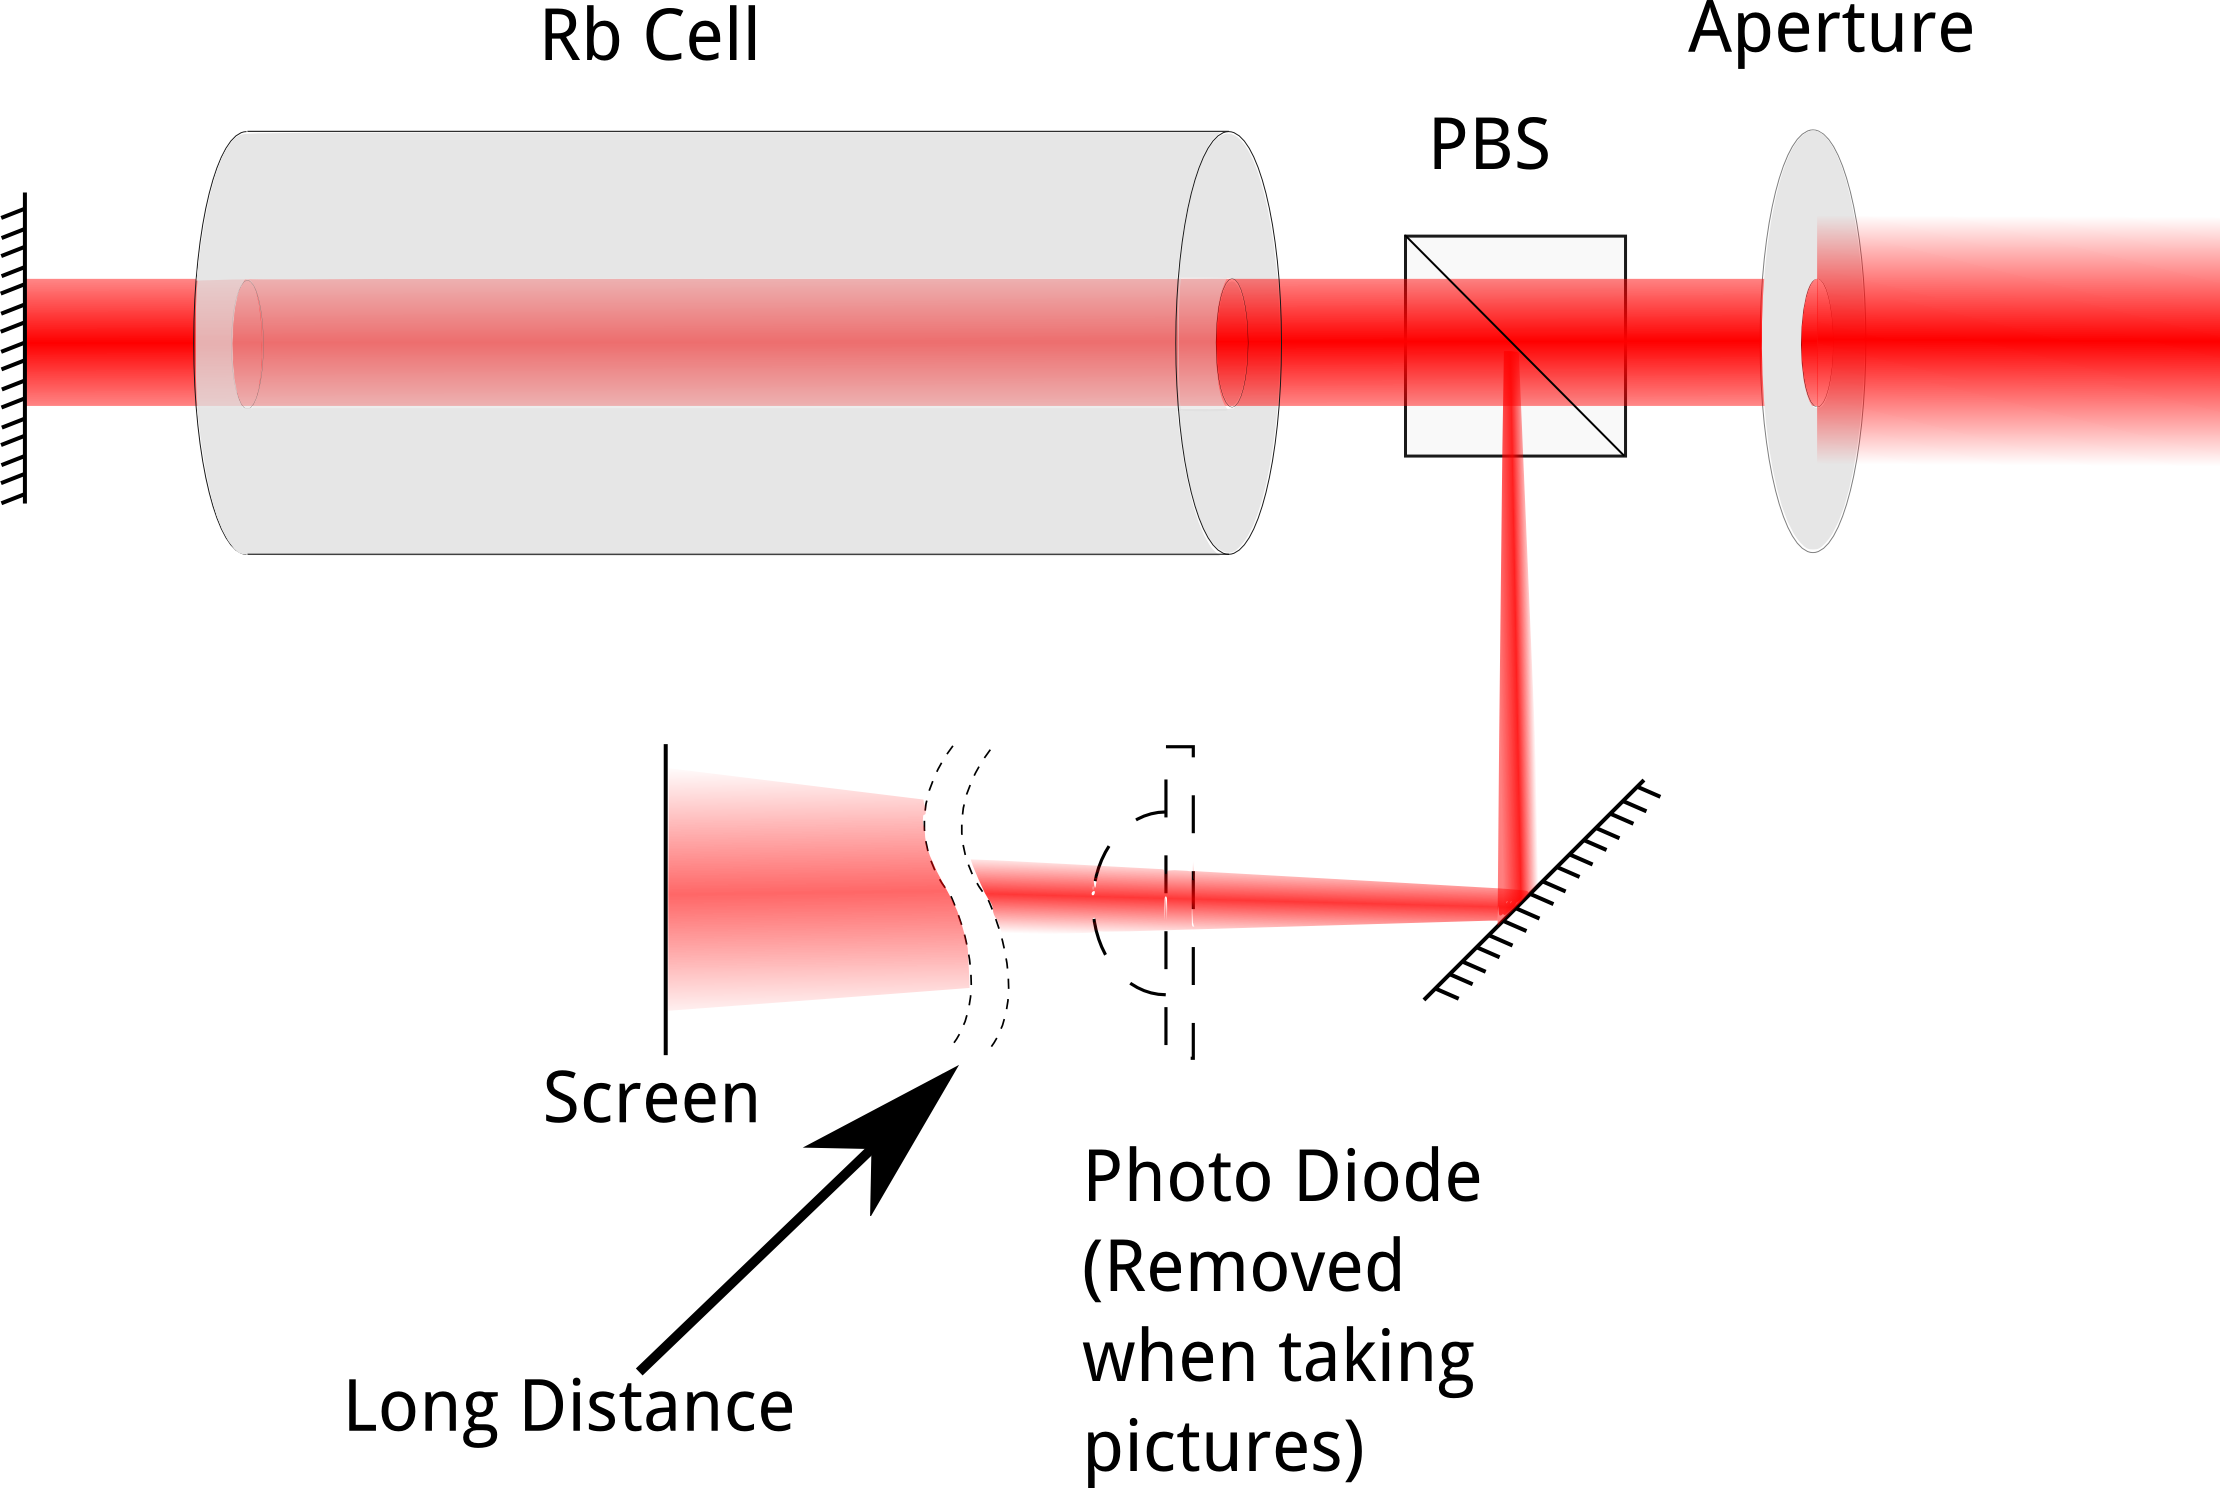
\includegraphics[width=9cm]{apparatus.png}
  \caption{Beam path setup of the experiment. The aperture is used to make the elliptical beam coming out of the diode laser more circular. The polarization beam splitter (PBS) is used to split the weak generated light with an orthogonal polarization from the main beam. A photo diode can be put in the beam path to measure the power helping to find the resonance frequency.}
  \label{apparatus}
\end{figure}
\subsection{Heater design.}
\subsection{Imaging system.}

\section{Measurements and results}
\subsection{Generated light in the orthogonal polarization.}
\begin{figure}
  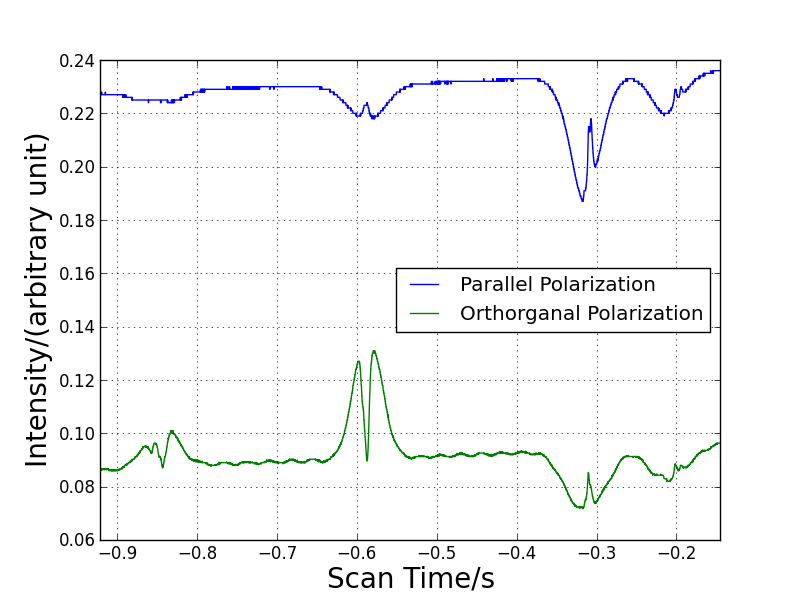
\includegraphics[width=9cm]{../data/5-16_csv/intensities.png}
  \caption{}
  \label{intensities}
\end{figure}

\subsection{Interference rings for red detuned light.}
\begin{figure}
  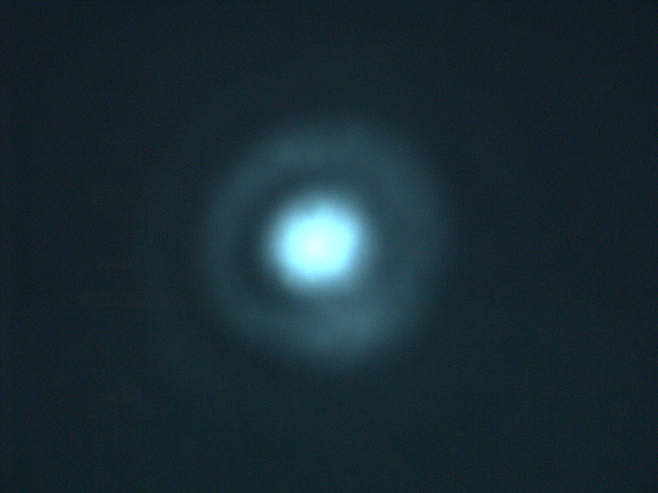
\includegraphics[width=7.8cm]{rings.png}
  \caption{}
  \label{rings}
\end{figure}
\begin{figure}
  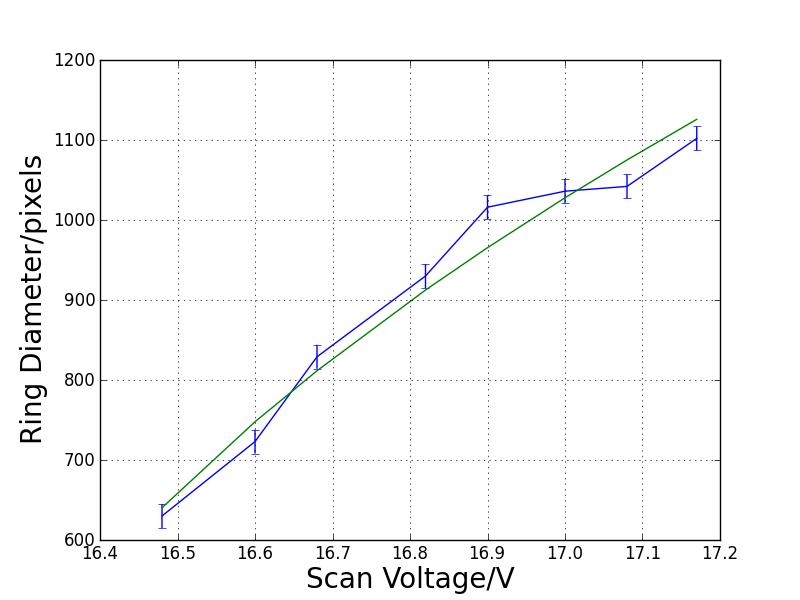
\includegraphics[width=9cm]{../data/5-16/ring-fit.png}
  \caption{}
  \label{ring_fit}
\end{figure}

\subsection{Flower like patterns}
\begin{figure}
  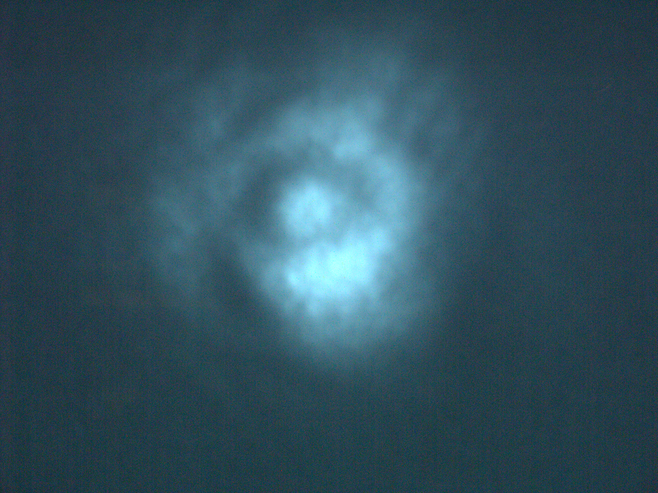
\includegraphics[width=7.8cm]{cone.png}
  \caption{}
  \label{cone}
\end{figure}
\begin{figure}
  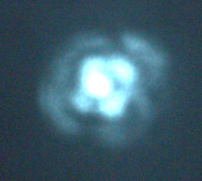
\includegraphics[width=7.8cm]{flower1.png}
  \caption{}
  \label{flower1}
\end{figure}
\begin{figure}
  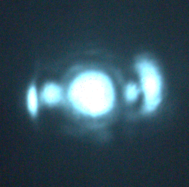
\includegraphics[width=7.8cm]{flower2.png}
  \caption{}
  \label{flower1}
\end{figure}
\begin{figure}
  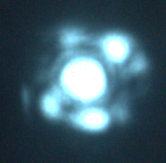
\includegraphics[width=7.8cm]{flower3.png}
  \caption{}
  \label{flower1}
\end{figure}

\section{Conclusion}

\bibliography{report}
\end{document}
